% !TEX root = ../main.tex
\chapter{Dynamic Mode Decomposition}\label{ch:dmd}
\begin{paracol}{2}

\begin{sources}
\begin{tabularx}{\linewidth}{@{}V l L@{}}
\toprule
\textbf{Video} & \textbf{Length} & \textbf{Content}\\
\midrule
\seg{4}{1}{V4.1 Dynamic Mode Decomposition (Overview)} & 18:18 & Snapshot matrices $X$, $X'$; the best-fit linear operator $A$; the algorithm (SVD, $\tilde A$, eigendecomposition, exact modes); truncation; prediction; DMD = PCA in space + Fourier in time.\\
\seg{4}{2}{V4.2 Dynamic Mode Decomposition (Examples)} & 7:43 & Connection to Koopman; extensions (compressed, multiresolution, control, randomized, streaming, denoising, extended); applications; the toy video: PCA vs ICA vs DMD.\\
\seg{4}{3}{V4.3 Dynamic Mode Decomposition (Code)} & 8:15 & The cylinder-wake code of the DMD book: singular values, rank $r=21$, modes, eigenvalues on the unit circle.\\
\seg{4}{4}{V4.4 Compressed Sensing and Dynamic Mode Decomposition} & 30:35 & Compressed sensing; compressive-sampling DMD (L1 reconstruction of modes) and compressed DMD (modes from the full $X'$); error analysis; invariance of DMD under unitary transformations.\\
\bottomrule
\end{tabularx}

\smallskip
\textbf{Transcripts} \file{materials/transcripts/C04-V0*.txt}.
\textbf{Book} Sec.~7.2 (DMD); Sec.~1.4--1.5 (SVD, pseudo-inverse, PCA); Ch.~3 (compressed sensing).
\textbf{Code} \file{code/ch04_dmd.py}, \file{ch04_cdmd.py}. The cylinder data of the videos are not
used (they are on dmdbook.com); a toy data set reproduces the same effects.
\end{sources}

\section*{Motivation}
DMD is the first data-driven method of the course and the most widely used. From a movie of a
high-dimensional system it extracts, purely from data, (a) a few spatial patterns, the \emph{modes}, and
(b) for each one a single complex frequency, i.e.\ a pure oscillation with exponential growth or decay;
together they form a linear reduced-order model \ts{4}{1}{0:02}. It needs no equations of motion: ``turn
the crank'' on any time-resolved data \ts{4}{1}{1:26}. For a physicist: it is a numerically robust way
to find the normal modes of a system you can only film.

% ------------------------------------------------------------------
\section{The DMD algorithm}\label{sec:dmd-algorithm}

\paragraph{History and scope.} DMD was introduced in fluid dynamics by Peter Schmid and later connected
to Koopman operator theory by Clancy Rowley, Igor Mezi\'c and collaborators \ts{4}{1}{0:44}. Since then it
has been applied to disease modelling, neuroscience, robotics, finance, plasmas \ts{4}{1}{1:05}, and it
works equally on experimental data such as PIV images \ts{4}{1}{1:46}.

\begin{history}[Schmid, Rowley, Mezi\'c]
P.~J.~Schmid presented DMD in 2008 and published it as \emph{Dynamic mode decomposition of numerical and
experimental data}, J.\ Fluid Mech.\ 656 (2010) 5--28. C.~W.~Rowley, I.~Mezi\'c, S.~Bagheri,
P.~Schlatter and D.~S.~Henningson, \emph{Spectral analysis of nonlinear flows}, J.\ Fluid Mech.\ 641
(2009) 115--127, showed that DMD approximates the eigenvalues and modes of the Koopman operator,
building on Mezi\'c's \emph{Koopman modes} (2005). The ``exact DMD'' used today is from J.~H.~Tu,
C.~W.~Rowley, D.~M.~Luchtenburg, S.~L.~Brunton and J.~N.~Kutz, J.\ Comput.\ Dyn.\ 1 (2014) 391--421.\par
\textit{References:} the papers cited; Kutz, Brunton, Brunton, Proctor, \emph{Dynamic Mode
Decomposition} (SIAM, 2016).
\end{history}

\paragraph{Step 1: data.} Take a movie of the flow, e.g.\ vortex shedding behind a cylinder, cut it into
snapshots $\vb x_1,\dots,\vb x_m$ (each a vorticity field with $\sim10^5$ values, reshaped into a tall
column), and arrange them in two matrices shifted by one time step \ts{4}{1}{2:07}\ts{4}{1}{2:48}\ts{4}{1}{3:29}:
\begin{equation}\label{eq:dmd-data}
  X=\begin{bmatrix}\vb x_1&\vb x_2&\cdots&\vb x_{m-1}\end{bmatrix},\qquad
  X'=\begin{bmatrix}\vb x_2&\vb x_3&\cdots&\vb x_m\end{bmatrix}.
\end{equation}
For fluids these are very tall and skinny: $n\sim10^5$--$10^9$ rows, $m\sim10^2$--$10^3$ columns
\ts{4}{1}{4:10}.

\paragraph{Step 2: the hypothesis.} Look for the best-fit linear operator with \ts{4}{1}{4:31}\ts{4}{1}{4:51}
\begin{equation}\label{eq:dmd-A}
  X'\approx AX,\qquad A=\operatorname*{argmin}_A\lVert X'-AX\rVert_F=X'X^{\dagger},
\end{equation}
where $X^\dagger$ is the Moore--Penrose pseudo-inverse. This does not claim that the dynamics is linear
(Navier--Stokes is not): $A$ simply has enough freedom to approximate the evolution of the data
\ts{4}{4}{2:51}. But $A$ is $n\times n$, a trillion entries for $n=10^6$: it cannot even be stored
\ts{4}{1}{5:12}\ts{4}{1}{5:32}.

\begin{definition}[New concepts: DMD eigenvalues and modes]\label{def:dmd}
The \textbf{dynamic mode decomposition} of the data \eqref{eq:dmd-data} is the set of leading eigenvalues
$\lambda_j$ (\textbf{DMD eigenvalues}) and eigenvectors $\boldsymbol\phi_j$ (\textbf{DMD modes}) of
$A=X'X^\dagger$, computed without forming $A$ \ts{4}{1}{5:52}\ts{4}{1}{14:07}. Each mode, reshaped, is a
spatial pattern (an ``eigen flow field'') that evolves in time as $\lambda_j^k$: a pure tone, a pure
exponential growth or decay, or a growing or decaying oscillation \ts{4}{1}{6:13}\ts{4}{1}{6:33}.
\end{definition}

\paragraph{Step 3: the algorithm.} If enough snapshots are collected, a few coherent patterns dominate,
even with a million degrees of freedom \ts{4}{1}{7:56}\ts{4}{1}{8:17}. The algorithm exploits this
\ts{4}{1}{8:37}--\ts{4}{1}{12:23}:
\begin{enumerate}
  \item \textbf{SVD}: $X=U\Sigma V^*$ (economy size), truncated to rank $r$: $U_r\in\C^{n\times r}$,
        $\Sigma_r$, $V_r$. The columns of $U$ are the POD modes, ordered by the variance they capture
        \ts{4}{1}{8:37}\ts{4}{1}{8:57};
  \item \textbf{projected operator}: with $A\approx X'V_r\Sigma_r^{-1}U_r^*$,
        \begin{equation}\label{eq:dmd-Atilde}
          \tilde A=U_r^*AU_r=U_r^*X'V_r\Sigma_r^{-1}\in\C^{r\times r},
        \end{equation}
        the best-fit linear dynamics of the POD coefficients \ts{4}{1}{9:18}\ts{4}{1}{9:59}\ts{4}{1}{10:41};
  \item \textbf{eigendecomposition}: $\tilde AW=W\Lambda$; the eigenvalues of $\tilde A$ are the nonzero
        eigenvalues of $A$ \ts{4}{1}{11:02}\ts{4}{1}{11:22};
  \item \textbf{exact DMD modes} (Tu et al.\ 2014, slightly different from Schmid's $U_rW$):
        \begin{equation}\label{eq:dmd-Phi}
          \Phi=X'V_r\Sigma_r^{-1}W
        \end{equation}
        \ts{4}{1}{11:42}\ts{4}{1}{12:03}.
\end{enumerate}
That is all: four or five lines of code, fast and scalable \ts{4}{1}{12:44}.

\begin{proposition}[Why the algorithm works]\label{prop:dmd-exact}
Let $A=X'V_r\Sigma_r^{-1}U_r^*$ (the best fit restricted to the span of $U_r$), $\tilde A=U_r^*AU_r$, and
$\tilde A\vb w=\lambda\vb w$ with $\lambda\neq0$. Then $\boldsymbol\phi=X'V_r\Sigma_r^{-1}\vb w$ satisfies
$A\boldsymbol\phi=\lambda\boldsymbol\phi$, and $\boldsymbol\phi\neq0$.
\end{proposition}
\begin{proof}
Note $\tilde A=U_r^*X'V_r\Sigma_r^{-1}$, so $U_r^*\boldsymbol\phi=\tilde A\vb w=\lambda\vb w$. Then
$A\boldsymbol\phi=X'V_r\Sigma_r^{-1}(U_r^*\boldsymbol\phi)=\lambda X'V_r\Sigma_r^{-1}\vb w=\lambda\boldsymbol\phi$.
If $\boldsymbol\phi=0$ then $\lambda\vb w=U_r^*\boldsymbol\phi=0$, impossible. Conversely every eigenvector
of $A$ with $\lambda\ne0$ lies in the range of $X'V_r$, so this gives all nonzero eigenvalues.
\end{proof}

\begin{intuition}[Lifting back with the data]
The small eigenvector $\vb w$ lives in POD-coefficient space; \eqref{eq:dmd-Phi} lifts it back to the
full space by taking a linear combination of the \emph{shifted} snapshots, columns of $X'$
\ts{4}{4}{6:38}. Schmid's projected modes $U_r\vb w$ are the projection of $\boldsymbol\phi$ onto the POD
subspace; the two coincide when the columns of $X'$ lie in the span of $X$.
\end{intuition}

\paragraph{Truncation.} With $r=m-1$ (exact SVD) one gets $m-1$ eigenvalues and modes. If the first,
say, five POD modes capture 99\% of the energy, keep $r=5$: a $5\times5$ $\tilde A$, five eigenvalues,
five modes \ts{4}{1}{13:06}\ts{4}{1}{13:27}. The rank $r$ is the main knob of DMD \ts{4}{3}{3:28}.

\paragraph{Prediction.} With $b_j$ the amplitude of each mode in the initial condition (e.g.\
$\vb b=\Phi^\dagger\vb x_1$) \ts{4}{1}{14:28},
\begin{equation}\label{eq:dmd-pred}
  \vb x_{k+1}\approx\sum_{j=1}^r b_j\lambda_j^{k}\boldsymbol\phi_j,
  \qquad\text{or}\qquad
  \vb x(t)\approx\sum_j b_j e^{\omega_jt}\boldsymbol\phi_j,\ \ \omega_j=\frac{\ln\lambda_j}{\Delta t}.
\end{equation}
This works well for periodic or quasi-periodic systems, even strongly nonlinear ones; strong transients,
intermittency or non-stationarity need fancier regressions and a nonlinear framework \ts{4}{1}{14:49}\ts{4}{1}{15:09}.

\begin{remark}[DMD is regression]
The key observation (J.~Tu): DMD \emph{is} a best-fit linear regression from $X$ to $X'$, so every
regression technique applies: noise-robust regression, sparsity-promoting regression, and so on
\ts{4}{1}{15:30}\ts{4}{1}{15:50}.
\end{remark}

\begin{intuition}[PCA and Fourier ``had a baby'']
The SVD step is PCA: it finds the fewest patterns that explain the data. Then a linear regression on the
principal components ($\tilde A$) is diagonalized to find linear combinations of them that each have a
single frequency in time. DMD is PCA in space plus the Fourier transform in time \ts{4}{1}{16:11}\ts{4}{1}{16:52}\ts{4}{1}{17:13}.
Unlike a Fourier transform, the frequencies are not fixed by the record length and can grow or decay.
\end{intuition}

\begin{keyformulas}
\begin{itemize}
  \item $X'\approx AX$, $A=X'X^\dagger$; $X=U_r\Sigma_rV_r^*$; $\tilde A=U_r^*X'V_r\Sigma_r^{-1}$;
        $\tilde AW=W\Lambda$; $\Phi=X'V_r\Sigma_r^{-1}W$.
  \item $\vb x_k\approx\Phi\Lambda^{k-1}\vb b$, $\omega_j=\ln\lambda_j/\Delta t$: $\operatorname{Re}\omega_j$
        growth rate, $\operatorname{Im}\omega_j$ angular frequency.
\end{itemize}
\end{keyformulas}

% ------------------------------------------------------------------
\section{Extensions, applications, and a toy example}\label{sec:dmd-examples}

\paragraph{Connection to Koopman.} Although DMD fits a linear model, it is connected to strongly
nonlinear dynamics: its eigenvalues and modes approximate those of the Koopman operator (Chapter~6)
\ts{4}{2}{0:23}\ts{4}{2}{0:44}.

\paragraph{Extensions.} Because DMD is linear regression, it is easily extended \ts{4}{2}{1:05}:
\begin{itemize}
  \item \textbf{compressed / compressed-sensing DMD}, for spatially under-resolved data, and compressed
        sensing in time for data that are not time resolved (\cref{sec:dmd-cs}) \ts{4}{2}{1:26};
  \item \textbf{multiresolution DMD} (N.~Kutz): DMD on a hierarchy of time windows, separating slow,
        medium and fast modes; it captures transient phenomena such as El Ni\~no \ts{4}{2}{1:46};
  \item \textbf{DMD with control} (J.~Proctor): identify the model while the system is actuated,
        $\vb x_{k+1}\approx A\vb x_k+B\vb u_k$ \ts{4}{2}{2:07};
  \item \textbf{randomized DMD} (N.~B.~Erichson and others) for very large data \ts{4}{2}{2:28};
  \item \textbf{streaming}, \textbf{denoising} and \textbf{extended} DMD (augmenting the measurements with
        nonlinear functions of them) \ts{4}{2}{2:48}\ts{4}{2}{3:09}.
\end{itemize}
Literally dozens of papers add innovations to the original algorithm \ts{4}{2}{3:29}.

\begin{application}[Where DMD is used]
Most DMD papers are in fluid dynamics (a jet in cross flow by Rowley, Mezi\'c et al., boundary layers,
combustion, shock--boundary-layer interaction), but also neuroscience, disease modelling, weather and
climate, robotics, finance, plasmas and video processing \ts{4}{2}{3:50}\ts{4}{2}{4:10}. The common
thread: high-dimensional data from a probably nonlinear, multiscale process with dominant coherent
structures \ts{4}{2}{4:31}.
\end{application}

\begin{casestudy}[A toy video: PCA, ICA and DMD]
B.~W.~Brunton's toy movie: $80\times80$ pixels (6400-dimensional data), with noise, in which two patterns
oscillate at different frequencies, a fast square and a slow Gaussian; without noise it is a rank-2
system \ts{4}{2}{4:51}\ts{4}{2}{5:12}\ts{4}{2}{5:33}.
\begin{itemize}
  \item \textbf{PCA} (the SVD) gets the rank right, 2, but its modes, ordered by energy, \emph{mix} the
        two frequencies \ts{4}{2}{5:53}\ts{4}{2}{6:14};
  \item \textbf{ICA} extracts two shapes corresponding to fast and slow, but they are noisy and there is no
        model of their time evolution \ts{4}{2}{6:35};
  \item \textbf{DMD} separates square and Gaussian cleanly, denoises them, and identifies the two
        frequencies: a linear dynamical model is under the hood \ts{4}{2}{6:55}\ts{4}{2}{7:15}.
\end{itemize}
\end{casestudy}

\codefile{DMD function and the toy video}{../code/ch04_dmd.py}

\begin{nfigure}
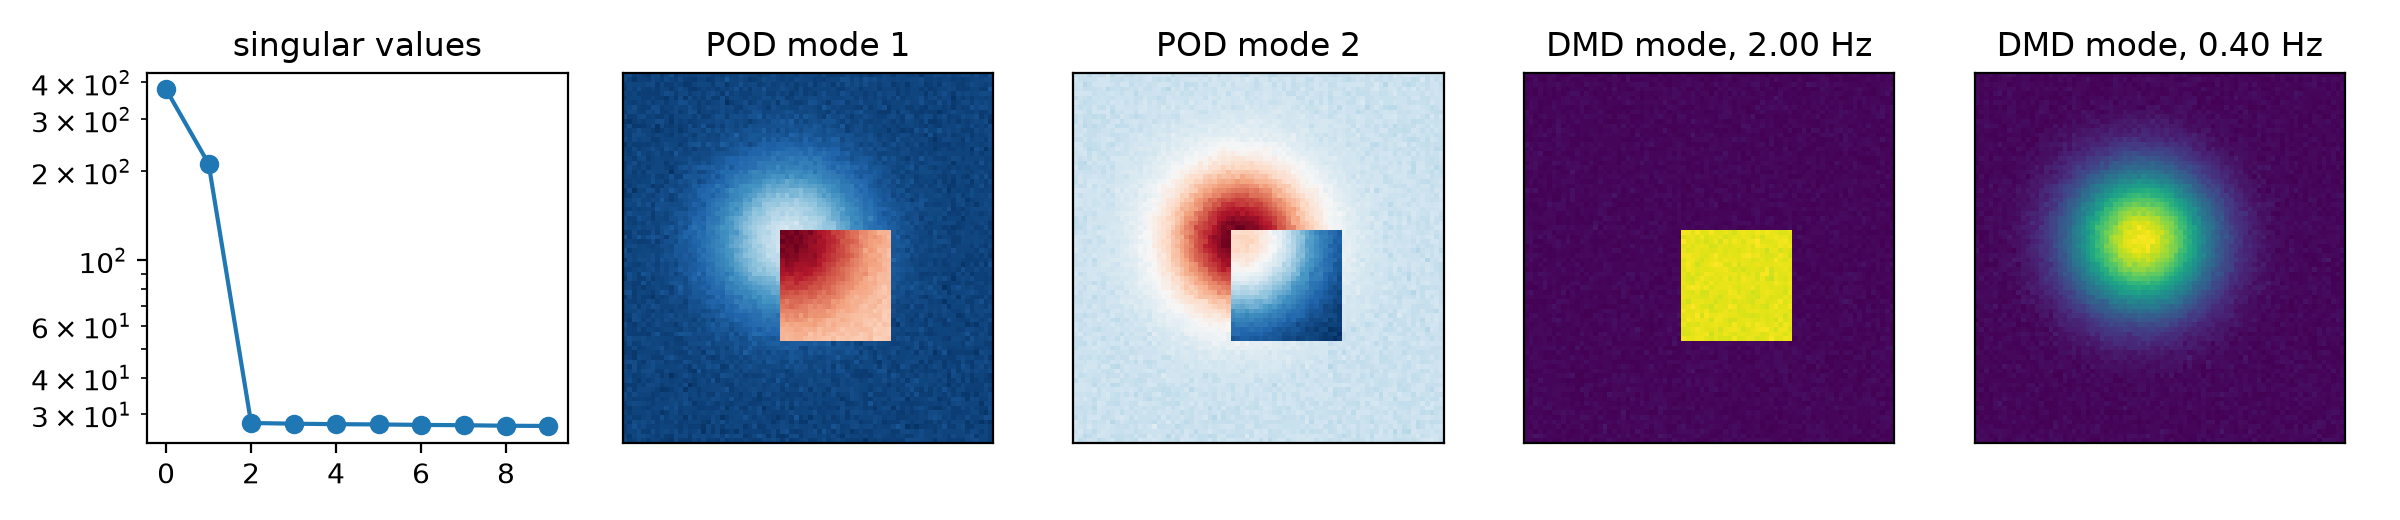
\includegraphics[width=\linewidth]{figures/ch04-dmd-toy.png}
\caption{Output of \file{ch04_dmd.py}. Singular values: rank 2 plus a noise floor. POD modes 1--2 mix
the square and the Gaussian (which overlap and are not orthogonal); the two DMD modes (modulus) separate
them, with the right frequencies, 2.00 and 0.40\,Hz, and growth rates $\approx0$ (the script prints
$-0.003$ and $-0.008\,\mathrm{s}^{-1}$, a small bias due to the noise).}\label{fig:dmd-toy}
\end{nfigure}

\begin{remark}[Noise bias]
With noise, DMD eigenvalues are biased towards the inside of the unit circle (spurious damping), because
least squares attributes all the noise to $X'$ and none to $X$. Remedies are noise-robust regressions:
forward--backward DMD, total-least-squares DMD, optimized DMD.
\end{remark}

% ------------------------------------------------------------------
\section{DMD in practice: the cylinder wake}\label{sec:dmd-code}

The code of the DMD book (dmdbook.com) for the flow past a cylinder \ts{4}{3}{0:22}\ts{4}{3}{1:04}:
\begin{enumerate}
  \item load the vorticity fields, one per column, and split them into $X$ (columns $1..m-1$) and $X'$
        (columns $2..m$) \ts{4}{3}{1:24}\ts{4}{3}{1:45};
  \item economy SVD of $X$ (a full SVD would be far too expensive) \ts{4}{3}{2:05};
  \item plot the singular values on a log scale, always a good idea \ts{4}{3}{2:05}: the first one is the
        mean flow (not subtracted), then they come in \emph{pairs}, the sine/cosine pairs of the periodic
        shedding and its harmonics \ts{4}{3}{2:47}\ts{4}{3}{3:08};
  \item truncate at $r=21$: the mean plus ten harmonic pairs \ts{4}{3}{3:28}\ts{4}{3}{3:48};
  \item compute $\tilde A$ ($21\times21$), its eigendecomposition and the modes $\Phi$, ``three lines''
        \ts{4}{3}{4:09}\ts{4}{3}{4:50}\ts{4}{3}{6:33};
  \item plot the modes: pairs oscillating at one frequency, finer and finer for higher harmonics
        \ts{4}{3}{5:32}\ts{4}{3}{5:52};
  \item plot the eigenvalues with the unit circle (discrete time): complex-conjugate pairs on the circle,
        which explains the sine/cosine pairs of modes oscillating out of phase \ts{4}{3}{6:53}\ts{4}{3}{7:14}.
\end{enumerate}
Here the DMD modes look much like the POD modes because the cylinder wake is a ``very normal'' system
\ts{4}{3}{5:52}\ts{4}{3}{6:12}.

\begin{secondary}[Why the modes come in pairs, and why DMD $\approx$ POD here]
A real travelling or rotating pattern $\operatorname{Re}(\boldsymbol\phi e^{i\omega t})=
\boldsymbol\phi_R\cos\omega t-\boldsymbol\phi_I\sin\omega t$ needs two real spatial fields, hence two
singular values of similar size and a conjugate pair $\lambda,\bar\lambda$. On the periodic attractor the
time coefficients of different harmonics are orthogonal over a period, so the SVD, which produces
orthogonal time series, cannot mix different frequencies, and the POD modes coincide (pairwise) with the
DMD modes. When the dynamics is non-normal or transient this fails, and DMD and POD differ.
\end{secondary}

% ------------------------------------------------------------------
\section{Compressed sensing and DMD}\label{sec:dmd-cs}

DMD needs a lot of data: acquiring and processing $X$, $X'$ can be expensive \ts{4}{4}{9:42}\ts{4}{4}{10:03}.
In PIV, for example, spatial and temporal resolution are limited by hardware: sometimes the data cannot
even be transferred from the camera to memory fast enough \ts{4}{4}{10:23}\ts{4}{4}{10:44}. Other uses of
sparsity in DMD: selecting few important modes (Jovanovi\'c et al.), sparse sampling in time (Tu et al.)
\ts{4}{4}{11:04}\ts{4}{4}{11:25}. Here: sparse sampling in \emph{space} \ts{4}{4}{11:46}.

\paragraph{Compressed sensing in one paragraph.} Most high-dimensional signals (images, flow fields,
audio) are \emph{sparse} in a suitable basis: in the Fourier domain most coefficients of an image are small
and can be dropped, which is how compression works \ts{4}{4}{12:06}\ts{4}{4}{12:27}\ts{4}{4}{12:48}.
Compressed sensing (about ten years old at the time of the video) turns this around: measure much less
and infer the sparse coefficients consistent with the measurements \ts{4}{4}{13:09}\ts{4}{4}{13:30}.

\begin{definition}[New concepts: sparsity, compressed sensing]\label{def:dmd-cs}
A vector $\vb x\in\R^n$ is $K$-\textbf{sparse} in a basis $\Psi$ if $\vb x=\Psi\vb s$ with at most $K$
nonzero entries in $\vb s$. Given $p\ll n$ measurements $\vb y=C\vb x=C\Psi\vb s$,
\textbf{compressed sensing} recovers $\vb s$ by the convex problem
\begin{equation}\label{eq:dmd-l1}
  \min_{\vb s}\lVert\vb s\rVert_1\quad\text{subject to}\quad\vb y=C\Psi\vb s
\end{equation}
instead of the combinatorial search for the sparsest $\vb s$ ($\ell_0$). It succeeds with high probability
if $p\gtrsim K\log(n/K)$ and the measurements are \emph{incoherent} with $\Psi$ (e.g.\ random), so that
$C\Psi$ satisfies the restricted isometry property: it acts almost like an isometry on sparse vectors
\ts{4}{4}{13:51}\ts{4}{4}{14:32}\ts{4}{4}{14:52}\ts{4}{4}{15:13}.
\end{definition}

The $\ell_1$ problem is a linear program: its cost grows polynomially, so Moore's law lets it keep up with
bigger data, which a brute-force search cannot \ts{4}{4}{15:13}\ts{4}{4}{15:33}. Example: measure 1\% of the
velocities of a flow at random points, infer its sparse Fourier coefficients, and fill in the other 99\%
\ts{4}{4}{16:15}\ts{4}{4}{16:36}.

\begin{history}[Compressed sensing]
Compressed sensing was founded in 2004--2006 by E.~Cand\`es, J.~Romberg and T.~Tao (\emph{Robust
uncertainty principles}, IEEE Trans.\ Inf.\ Theory 52, 2006) and D.~Donoho (\emph{Compressed sensing},
same journal and year). An early inspiration: Cand\`es reconstructed a Shepp--Logan phantom image almost
exactly from very few Fourier samples using $\ell_1$ (total-variation) minimization. The figure used in the
video is from R.~Baraniuk, \emph{Compressive sensing}, IEEE Signal Process.\ Mag.\ (2007).\par
\textit{References:} the papers cited; Brunton \& Kutz, Ch.~3.
\end{history}

\paragraph{Two algorithms.} With a measurement matrix $C\in\R^{p\times n}$ (e.g.\ random pixels), the
compressed data are $Y=CX$, $Y'=CX'$ \ts{4}{4}{17:39}\ts{4}{4}{17:59}.
\begin{enumerate}
  \item \textbf{Compressive-sampling (compressed-sensing) DMD}: only $Y,Y'$ exist (sparse sensors, or
        trading spatial for temporal resolution). Do DMD on $Y,Y'$, getting $\Lambda_Y$, $\Phi_Y$, then
        reconstruct each full mode by \eqref{eq:dmd-l1} with $\boldsymbol\phi_Y=C\Psi\vb s$
        \ts{4}{4}{18:20}. On the cylinder, $\sim1000$ measurements of a $\sim10^5$-dimensional state (1\%)
        reconstruct the leading modes well and the higher ones with some noise; the eigenvalues are almost
        exact, $\Lambda_X\approx\Lambda_Y$ to near machine precision \ts{4}{4}{18:41}\ts{4}{4}{19:01}.
  \item \textbf{Compressed DMD}: the full data exist but the SVD is too expensive. Compress, do DMD on
        $Y,Y'$, and get the full modes with no $\ell_1$ at all, as
        \begin{equation}\label{eq:dmd-cdmd}
          \Phi_X\approx X'V_Y\Sigma_Y^{-1}W_Y ,
        \end{equation}
        linear combinations of the columns of the full $X'$ \ts{4}{4}{19:43}\ts{4}{4}{20:24}. On the cylinder
        21 random pixels already give the first mode, 40 give all of them \ts{4}{4}{20:45}; cluster-sized
        computations fit on a laptop \ts{4}{4}{21:25}.
\end{enumerate}
The decision: only subsampled data $\Rightarrow$ compressive-sampling DMD with $\ell_1$; full data but slow
$\Rightarrow$ compressed DMD \ts{4}{4}{21:47}\ts{4}{4}{22:28}. With enough buoys in the ocean one could
infer the DMD of a high-resolution sensor network \ts{4}{4}{23:09}. In the error analysis on a double-gyre
flow, the mode error of compressed-sensing DMD decreases slowly (low at $\sim1000$ measurements, 1\%),
that of compressed DMD much faster (very good at $\sim100$) \ts{4}{4}{23:29}\ts{4}{4}{24:10}\ts{4}{4}{24:31}.

\codefile{compressed DMD on the toy video}{../code/ch04_cdmd.py}

The script prints, for $p=20,100,400$ random pixels out of 6400: eigenvalue errors $0.9$,
$1.4\times10^{-2}$, $5\times10^{-3}$ and mode errors $(0.41,0.16)$, $(0.02,0.01)$, $(0.008,0.005)$. With 20
pixels too few of them fall on the square and the Gaussian, which are \emph{localized}: in the pixel basis
these signals are not incoherent with point measurements. 100 pixels (1.6\%) are enough.

\paragraph{Why it works.} Three facts \ts{4}{4}{24:51}:
\begin{enumerate}
  \item DMD is invariant under \emph{right} unitary transformations: shuffling the columns of $X$ and of
        $X'$ in the same way gives the same eigenvalues and modes, because the SVD is invariant
        \ts{4}{4}{25:12}\ts{4}{4}{25:33};
  \item DMD is almost invariant under \emph{left} unitary transformations: if $Y=CX$, $Y'=CX'$ with $C$
        unitary (permuting rows, a spatial FFT, a POD basis), the eigenvalues are the same and the modes are
        $\Phi_Y=C\Phi_X$ \ts{4}{4}{25:53}\ts{4}{4}{26:13}\ts{4}{4}{26:34}\ts{4}{4}{26:54};
  \item a compression $C\in\R^{p\times n}$ is not unitary, but if the data are sparse, $X=\Psi S$, compressed
        sensing gives conditions under which $C\Psi$ acts like an isometry on sparse vectors, which is
        all that is needed \ts{4}{4}{27:35}\ts{4}{4}{27:56}\ts{4}{4}{28:17}\ts{4}{4}{28:59}.
\end{enumerate}

\begin{proof}[Proof of fact 2]
If $Y=CX$ with $C^*C=I$, then $Y=(CU)\Sigma V^*$ is an SVD of $Y$, so $U_Y=CU$, $\Sigma_Y=\Sigma$, $V_Y=V$.
Then $\tilde A_Y=U^*C^*CX'V\Sigma^{-1}=\tilde A_X$, so same $\Lambda$ and $W$, and
$\Phi_Y=CX'V\Sigma^{-1}W=C\Phi_X$.
\end{proof}

The code of the paper (a sparse dynamical system on a torus driving five spatial Fourier coefficients) is
available to try different compression ratios and samplings \ts{4}{4}{29:20}\ts{4}{4}{29:40}.

\section*{Exercises}

\begin{exercise}[DMD of a linear system]
Generate data from $\vb x_{k+1}=A\vb x_k$ with a random $A\in\R^{50\times50}$ of rank 4 (scaled so that its
eigenvalues have modulus $\le1$). Show numerically that DMD with $r=4$ recovers the nonzero eigenvalues of
$A$ exactly. What happens with $r=6$? With noise?
\end{exercise}

\begin{exercise}[Pseudo-inverse]
Show that $A=X'X^\dagger$ minimizes $\lVert X'-AX\rVert_F$, and that among the minimizers it has the smallest
Frobenius norm. Write $X^\dagger$ via the SVD.
\end{exercise}

\begin{exercise}[One real oscillation needs two modes]
Take data $x(t)=\cos(\omega t)\,\vb f$ for a fixed spatial vector $\vb f$. What is the rank of $X$? Can
DMD find the frequency? Now take $\vb f\cos\omega t+\vb g\sin\omega t$ with $\vb f\perp\vb g$: show that
$r=2$ gives $\lambda=e^{\pm i\omega\Delta t}$. Relate this to the singular-value pairs of the cylinder.
(This is the reason \file{ch04_dmd.py} uses complex data; Chapter~8 gives another cure: time delays.)
\end{exercise}

\begin{exercise}[Mean subtraction]
Run DMD on the toy data plus a constant background. Show that the mean appears as a mode with
$\lambda=1$. What happens to DMD if the mean is subtracted first? (Hint: Chen, Tu, Rowley 2012 show that
mean-subtracted DMD reduces to a temporal DFT.)
\end{exercise}

\begin{exercise}[Left-unitary invariance]
Verify fact 2 numerically on the toy data with $C$ the 2D FFT (normalized) and with a random orthogonal
$C$. Then try a random Gaussian $C\in\R^{p\times6400}$ and plot the eigenvalue error versus $p$.
\end{exercise}

\end{paracol}
